% reworked from http://www.texample.net/tikz/examples/decision-tree/
\tikzset{
  treenode/.style = {shape=rectangle, rounded corners,
                     draw, align=center,
                     top color=white, bottom color=blue!20},
  env/.style      = {treenode, font=\ttfamily\normalsize},
}

\begin{center}
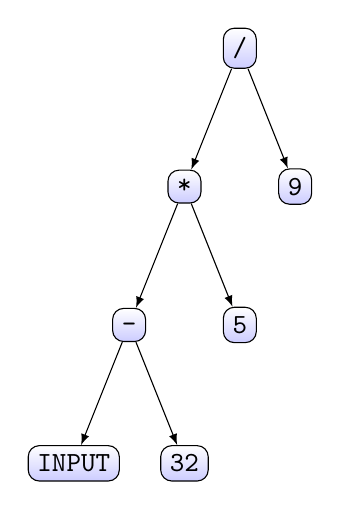
\begin{tikzpicture}
[
	grow                    = down,
	sibling distance        = 4em,
	level distance          = 5em,
	edge from parent/.style = {draw, -latex},
	every node/.style       = {font=\footnotesize},
	sloped
]
\node [env] {/}
	child
	{
		node [env] {*}
		child { 
			node [env] {-}
			child { node [env] {INPUT} }
			child { node [env] {32} }
			}
		child { node [env] {5} }
	}
	child { node [env] {9} }
	;

\end{tikzpicture}
\end{center}
